%\motto{Use the template \emph{chapter.tex} to style the various elements of your chapter content.}
\chapter{Physikalische Grundlagen}
\label{physics} % Always give a unique label

\chapterauthor{Amanda Hagan, Lucie Hartmann, Leon Lukacin, Ole Pross}

\abstract{some abstract}

\section{(Einführung in die Quantenmechanik für das Quantencomputing)}
\subsection{Motivation und Abgrenzung zur klassischen Physik }
\subsection{Wichtige Konzepte der Quantenmechanik }
\label{Wichtige Konzepte der Quantenmechanik}

\subsubsection*{\textit{Welle-Teilchen-Dualismus}}
\label{Welle-Teilchen-Dualismus}

In der Vergangenheit wurde in der Physik darüber diskutiert, ob Licht sich wie Teilchen oder wie Wellen verhält. Verschiedene Experimente lieferten Argumente für beide Seiten. Die Entdeckung des Elektromagnetismus sprach für Licht als Wellen. Die Beobachtung des photoelektrischen Effektes hingegen lieferte wieder Argumente, welche für Licht als Teilchen, als Photonen, sprachen. Aus diesen verschiedenen Entdeckungen leitete sich das Konzept des Welle-Teilchen-Dualismus ab. (vgl. \cite[Ch. 1.3.2]{kasirajan_fundamentals_2021})\\

Der Welle-Teilchen-Dualismus ist eines der fundamentalen Konzepte der Quantenmechanik. Es beschreibt, dass subatomare Teilchen wie Photonen oder Elektronen gleichermaßen Wellen- und Teilcheneigenschaften besitzen. Dies widerspricht den Konzepten der klassischen Physik, in der Wellen und Teilchen getrennte Kategorien darstellen. (vgl. \cite[Ch. 2]{schmitz_particles_2022})\\

Das zentrale Experiment zum Nachweis des Welle-Teilchen-Dualismus ist das Doppelspaltexperiment. Dabei wird ein Strom Photonen durch zwei eng beieinanderliegende Spalte (Doppelspalt) auf einen dahinterliegenden Schirm gelenkt. Dabei entsteht auf dem Schirm ein Interferenzmuster. Dies ist ein Effekt typisch für  Wellen, die Interferenz ist dabei die Überlagerung der Amplituden einzelner Wellen. Der Welleneffekt mit dem Interferenzmuster bleibt sogar bestehen wenn die Teilchen einzeln abgeschossen werden.\\
Daraus kann gefolgert werden, dass Teilchen sich wie Wellen verhalten, welche durch die beiden Spalten miteinander inferieren. Das Interferenzmuster verschwindet allerdings bei dem Versuch den Weg eines Teilchens durch Messung zu bestimmen. In diesem Fall der Messung verhält sich das Teilchen klassisch, wie man es von einem Teilchen erwarten würde und der Welleneffekt gehtegidnör verloren.\\
Somit konnte in dem Experiment neben dem Verhalten als Teilchen und Welle nachgewiesen werden, dass der Akt der Messung den Zustand des eines Objektes in einem quantenmechanischen System beeinflusst, ein Thema auf das später näher eingegangen wird.

\subsubsection*{\textit{Heisenbergsche Unschärferelation}}
\label{Heisenbergsche Unschärferelation}

Die Heisenbergsche Unschärferelation ist ein weiteres zentrales Prinzip der Quantenmechanik und wurde 1927 von Werner Heisenberg formuliert. Sie beschreibt eine fundamentale Grenze der gleichzeitigen Bestimmbarkeit bestimmter Paare von physikalischen Größen.\\
Betrachtet man beispielsweise den Ort- und Impuls eines Teilchens, so kann man diese beiden Eigenschaften nicht bis zu einer beliebigen Genauigkeit hin messen. Die Unschärferelation sagt nicht aus, dass Messgeräte zu ungenau sind um diese Werte zu bestimmen, sondern dass die Unschärfe eine fundamentale Eigenschaft der Quantenmechanik ist.\\
Sie resultiert aus der Wellencharakteristik von Teilchen in der Quantenmechanik. Je genauer der Ort durch eine bestimmte Wellenfunktion ermittelt wird, desto größer ist die Breite an Werten für den Impuls des Teilchens. Es muss bei einer solchen Messung also immer eine Abwägung zwischen den Werten stattfinden. \\
Die Unschärferelation stellt damit eine Abkehr vom Determinismus der klassischen Physik dar, in dem alle physikalischen Größen beliebig genau bestimmt werden können. Stattdessen legt die Unschärferelation die Grundlage für die probabilistische Natur quantenmechanischer Systeme und Zustände. (vgl. \cite[Ch. 1.6.3]{kasirajan_fundamentals_2021})

\subsubsection*{\textit{Zustände und Wellenfunktion}}
\label{Zustände und Wellenfunktion}

Ein Zustand beschreibt in der Physik die Menge aller physikalisch relevanten Informationen, die ein spezifisches System charakterisieren.\\
\\
In der klassischen Mechanik wird der Zustand eines Objektes, im einfachsten Fall eines einzelnen Teilchens, über den Ort und Impuls des Objektes beschrieben. Aus diesen Informationen lassen sich alle physisch messbaren Eigenschaften des Teilchens berechnen. Dieses Modell zur Zustandsbeschreibung reicht aufgrund von Quantenmechanischen Phänomenen allerdings nicht mehr aus, um auch Quantenobjekte und -systeme vollständig zu beschreiben. (vgl. \cite[Ch. 3.1]{osada_introduction_2022})\\

Der Zustand eines Quantenobjektes ist über die Wellenfunktion mit dem Symbol $\Psi$ (Psi) vollständig definiert. Die Wellenfunktion ist eine komplexe Funktion, ihre Funktionswerte stammen also aus dem Zahlenraum $\mathbb{C}$.\\
Die Wellenfunktion sagt aus, dass in einem durch sie beschriebenen Quantensystem die Wahrscheinlichkeitsdichte $P(x)$ das untersuchte Teilchen in dem Zustand $\Psi(x)$ an der Stelle $x$ zu finden $|\Psi(x)|^2$ beträgt. Es gilt also:\\
\begin{equation*}
P(x) = |\Psi(x)|^2
\end{equation*}
Dies ist notwendig, damit man als Ergebnis für die Wahrscheinlichkeit eine reale nicht negative Zahl erhält. Die Wellenfunktion wird immer normalisiert. Dies ist der Fall, da die Summe der Wahrscheinlichkeiten das Teilchen an irgendeinem Ort zu finden zusammengerechnet 1 ergeben muss.\\
Dieser Zusammenhang wird als erstes Postulat der Quantenmechanik bezeichnet. (vgl. \cite[Ch. 1.6]{kasirajan_fundamentals_2021})

\subsubsection*{\textit{Observable und Messung}}
\label{Observable und Messung}

Bei der Messung in einem Quantensystem können eine Vielzahl verschiedener Eigenschaften bestimmt werden.\\
Die mathematische Darstellung der Messergebnisse  wird  durch einen Operator ausgedrückt, welcher als Observable bezeichnet wird.\\
Ein Observable wird immer mit dem Symbol $\hat{V}$ dargestellt.
Observable Operatoren können für eine Vielzahl von Messungen definiert werden, beispielsweise für den Ort, den Impuls oder die Energie. Eine Ausnahme bildet die Zeit, welche in der Quantenmechanik nicht als Operator genutzt wird.\\
Obervables werden jeweils immer über eine Eigenvalue-Gleichung beschrieben. Diese hat die Form:
\begin{equation*}
\hat{V} \Psi = v \Psi
\end{equation*}
$\hat{V}$ ist dabei der Observable Operator und v das Eingenvalue, welches aus der Messung bestimmt wird. (vgl. \cite[Ch. 1.9.1]{lvovsky_quantum_2018})

\subsubsection*{\textit{Zeitentwicklung und Schrödingergleichung}}
\label{Zeitentwicklung und Schrödingergleichung}

Die Schrödingergleichung definiert die Zeitentwicklung einer Wellenfunktion $\Psi$. Sie beschreibt also wie sich ein Quantensystem im Verlauf der Zeit entwickelt. Die zeitabhängige Schrödingergleichung hat die Form:
\begin{equation*}
i\hbar \frac{\partial \Psi}{\partial t} = \hat{H} \Psi(x,t)
\end{equation*}
Wobei $i$ die imaginäre Einheit ist, $\hbar$ das reduzierte Planksche Wirkungsquantum und damit eine Konstante. $\frac{\partial \Psi}{\partial t}$ ist die Ableitung nach der Zeit $t$. Wie an der Darstellung zu erkennen ist, ist $\hat{H}$ ein Observable. Dieses wird als Hamiltonoperator bezeichnet und entspricht der Gesamtenergie des Quantensystems.\\
Die Schrödingergleichung liefert ein deterministisches Ergebnis für zukünftige Zuständes des Quantensystems. Das bedeutet ausgehend von einem Ausgangszustand gegeben durch eine Wellenfunktion lassen sich zukünftige Zustände durch die Schrödingergleichung berechnen. (vgl. \cite[Ch. 4.1]{osada_introduction_2022})

\section{Zentrale Quantenphänomene }

\subsection{Superposition }
\label{sec: Superposition}

Das Konzept der Superposition spielt eine zentrale Rolle in der Quantenmechanik. Die Superposition der Quantenmechanik unterscheidet sich maßgeblich von der Superposition der klassischen Physik.\\
Die quantenmechanische Superposition besagt, dass sich ein Quantensystem gleichzeitig in mehreren möglichen Zuständen befindet. Es wird von einer Überlagerung der Zustände gesprochen. Dieser überlagerte Zustand hält an, bis eine Messung durchgeführt wird.\\
Mathematisch wird dies durch die Überlagerung der jeweiligen Wellenfunktionen beschrieben, also der Linearkombination der Wellenfunktionen der einzelnen Zustände. Dabei entstehen neue Wellenfunktionen. Die Zustände haben dabei jeweils einen eigenen Wahrscheinlichkeitsanteil.\\
Bei der Messung erfolgt der Kollaps dieser Wellenfunktion in einen eindeutigen Zustand. Beim Kollaps der Wellenfunktion ist der gemessene Zustand von dieser Wahrscheinlichkeit abhängig. Ein Teilchen, zum Beispiel ein Elektron, kann sich somit in einer Überlagerung verschiedener Orte und Impulse befinden. Nach der Heisenbergschen Unschärferelation ist es dabei prinzipiell nicht möglich, beide Eigenschaften gleichzeitig exakt zu bestimmen. Erst bei einer Messung des Teilchens und dem Kollaps der Wellenfunktion lässt sich ein Wert ermitteln.\\

Es gibt mehrere Beispiele, um das Prinzip der Superposition zu verdeutlichen. Das bekannteste Gedankenexperiment zur Veranschaulichung der Superposition ist das von Schrödingers Katze: Dabei wird eine Katze zusammen mit einem Behältnis voll Gift und einer Strahlenquelle in eine nicht einsehbare Box gesperrt. Ein Mechanismus in der Box zerstört das Behältnis, wenn der zufällige Zerfall eines radioaktiven Teilchens der Strahlenquelle detektiert wird.\\
Die Katze befindet sich, solange keine Beobachtung erfolgt, aus Sicht des Betrachters in einer Superposition aus lebendig und tot. Also in einer Überlagerung mehrerer Zustände gleichzeitig. Gleichzeitig sind die Quantenzustände der Katze und des zerfallenden Atoms, welches das Austreten des Giftes verursacht hängen zusammen, es wird hierbei von Verschränkung (engl. ``entanglement'') gesprochen. Auf dieses Thema wird in Kapitel 1.2.3 näher eingegangen. (vgl. \cite[Ch. 2.1.3]{homeister_quantum_2022-1})\\
Ein anderes, sehr stark vereinfachtes, Gedankenexperiment zur Darstellung ist ein Münzwurf. Bei einem Münzwurf ist die Münze während sie in der Luft ist in einer Superposition aus den Zuständen Kopf und Zahl. Erst bei der Messung, beim Fangen der Münze, wird ein eindeutiger Zustand ermittelt.\\

\subsection{Quanteninterferenz}
\label{sec: Quanteninterferenz}

Wellen haben einige besondere Eigenschaften, da wie im Doppelspaltexperiment bewiesen, auch Quantenobjekte Welleneigenschaften haben sind diese relevant. An bestimmten Stellen kommt es bei Wellen zur Überlagerung, man spricht hierbei von Interferenz.


An diesen Punkten ist die Amplitude der Welle die Summe der Amplituden der vorherigen einzelnen Wellen. Es wird dabei zwischen konstruktiver Interferenz und destruktiver Interferenz unterschieden. Bei konstruktiver kommt es zur Verstärkung der Welle und bei destruktiver zu einer Abschwächung. Es ist sogar möglich, dass eine Welle durch destruktive Interferenz komplett zerstört wird. Diese Arten von Überlagerungen sind in Abbildung ~\ref{fig:Interferenz_Konstruktiv} und Abbildung~\ref{fig:Interferenz_Destruktiv} dargestellt. (vgl. \cite[Ch. 2.1.3]{schmitz_particles_2022})


Das Muster das beim Aufeinandertreffen von zwei Wellen entsteht, wird als Interferenzmuster bezeichnet. Dieses Phänomen war beim Doppelspaltexperiment von besonderer Bedeutung, da es ein weiterer Beweis für die Welleneigenschaften des Lichtes war.\\
Mathematisch überlagern sich durch Quanteninterferenz die Wahrscheinlichkeitsamplituden von Wellenfunktionen. Die Quanteninterferenz kann damit einen Einfluss auf die berechnete Wahrscheinlichkeit haben.
\\
\begin{figure}[H]
    \centering
    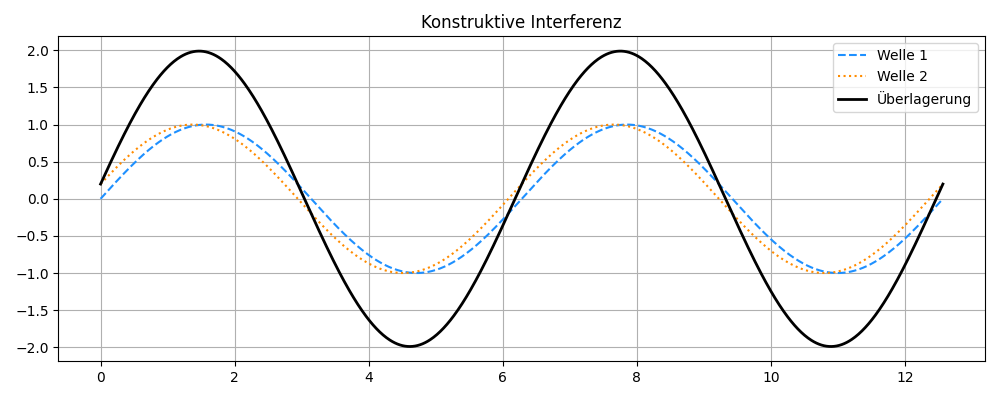
\includegraphics[width=1\linewidth]{images/physics/Interferenz_Konstruktiv.png}
    \caption{Konstruktive Interferenz zwischen zwei Wellen}
    \label{fig:Interferenz_Konstruktiv}
\end{figure}

\begin{figure}[H]
    \centering
    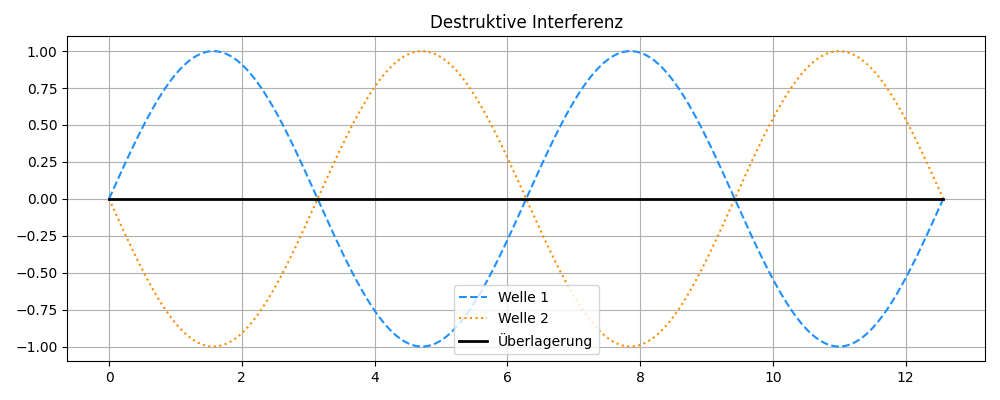
\includegraphics[width=1\linewidth]{images/physics/Interferenz_Destruktiv.png}
    \caption{Destruktive Interferenz zwischen zwei Wellen}
    \label{fig:Interferenz_Destruktiv}
\end{figure}

\subsection{Verschränkung }
\label{sec: Verschränkung}

Das Konzept der Verschränkung (engl. ``entanglement'') beschreibt gewissermaßen die Korrelation mehrerer Qubits miteinander, das heißt sie hängen in einem besonderen Maße zusammen. \\
Für einen erleichterten Einstieg soll ein Beispiel anhand zweier gewöhnlicher Münzen gemacht werden. Werden zwei gewöhnliche Münzen geworfen, hat man vier mögliche Ausgänge für den Münzwurf, bei denen H für Kopf und T für Zahl stehen sollen: HH, HT, TH, TT. \\
Alle Varianten der Ausgänge haben hierbei eine identische Wahrscheinlichkeit von 25\%. Sind diese zwei Münzen jedoch in einem verschränkten Zustand  $\frac{1}{\sqrt{2}} (\ket{HH} + \ket{TT})$, sind hierbei nur zwei Ausgänge möglich, die beide jeweils eine 50\%-Wahrscheinlichkeit haben, nämlich HH oder TT. \\
  
Diese Verschränkung ist unabhängig von der räumlichen Nähe der Münzen und kann über große Distanzen hinweg wirken. Weiß man das Ergebnis der einen Münze, so weiß man automatisch auch immer das Ergebnis der anderen Münze. Im Bereich der Quantenmechanik ist genau dies bezogen auf diverse Teilchen anstelle der Münzen möglich. 
Das Phänomen der Verschränkung ist jedoch ein reines Quantenphänomen, das keine Erklärung in der klassischen Physik besitzt. \\

Eine Vermutung über die Natur der Verschränkung besteht aus der sofortigen Informationsübertragung zweier Teilchen, die über die Schnelligkeit der Lichtgeschwindigkeit hinausgeht, was jedoch als widerlegt gilt. Stattdessen teilen Teilchen nicht-klassische Information während der Verschränkung, die im Messprozess beobachtet werden kann. \\ 

Eine weitere frühe Interpretation, bekannt unter dem Namen ``Hidden Variable Theory'', nahm an, dass Teilchen beim Erzeugen mit verbogenen Eigenschaften erschaffen werden, die Messergebnisse deterministisch bestimmen. Beispielsweise wäre hierfür der Zerfall eines Teilchens in zwei Teilchen. Auf Basis der Impulserhaltung kann man durch die Messung des Impuls des einen Teilchens auf den Impuls des anderen Teilchens schließen, da der Gesamtimpuls vorher bekannt ist. 
(vgl. \cite[Ch. 7]{hughes_quantum_2021})
% Quantum Computing for the Quantum Curious - Hughes et al. - 2021
\\ 

Das Problem dieser Theorie findet sich jedoch in Bell's Theorem, das zeigt, dass wenn die Welt durch diese versteckten Variablen beschrieben wäre, gewisse mathematische Ungleichungen in Experimenten eingehalten werden müssten. 
Diese gelten als Einschränkungen für alle lokal-realistischen Theorien, d.h. Theorien, die annehmen, dass Lokalität und Realismus gelten. \\ 
Lokalität bedeutet hierbei, dass es keinen Einfluss gibt, der sich schneller als mit Lichtgeschwindigkeit ausbreiten kann. \\
Realismus bezieht sich auf die Annahme, dass physikalische Größen zu jedem Zeitpunkt definierte Werte besitzen, unabhängig davon, ob diese gemessen werden. \\

Die quantenmechanische Verschränkung erfüllt diese Annahmen durch die ``spukhafte Fernwirkung'' jedoch nicht, da es eine scheinbar unmittelbare Verbindung über sehr große Distanz hinweg gibt. Dem Lokalitätsprinzip entsprechend, könnten zwei Systeme sich nur dann beeinflussen, wenn sie einen Kontakt oder ein physikalisches Feld haben, das sie verbindet. Quantenobjekte haben jedoch durch die mangelnde Lokalität keine klassische Kausalität, sondern nur die Beobachtung, dass die Ergebnisse immer korrelieren, auch wenn sie räumlich weit voneinander getrennt sind.
\\ 

Da die Grenzen der Bell-Ungleichung also nicht auf gemessene Experimente zutreffen, kann keine lokal-realistische Theorie das quantenmechanische Phänomen der Verschränkung erklären. Die Resultate stimmen mit der Quantenmechanik überein, anstatt mit lokalen Theorien wie der Hidden Variable Theory. 
\\ 

Basierend hierauf ergibt sich das Dilemma, dass Realismus und Lokalität nicht beide gleichzeitig gelten können. Diese Schlussfolgerung führt jedoch zu tiefergehenden philosophischen Fragen über die Realität, die an dieser Stelle nicht weiter behandelt werden sollen. Unabhängig davon findet die Verschränkungen Anwendungen in moderner Quantentechnologie, wie in der Quantenkryptographie oder Quanten-Teleportation.  
(vgl. \cite[Ch. 2.11]{homeister_quantum_2022-1})
%% Quantum Computing verstehen: Grundlagen - Anwendungen - Perspektiven - Homeister - 2022
\\

Um ein Beispiel für die Quantenverschränkung in der Praxis zu machen, soll an dieser Stelle noch  die spontane parametrische Fluoreszenz (engl. ``spontaneous parametric down-conversion, SPDC'') genannt werden. Bei diesem Prozess trifft ein Photon aus einem Laser auf ein nichtlineares Kristallmaterial. Dadurch spaltet sich das Photon in zwei neue Photonen, wobei die Polarisation der neuen Photonen miteinander verschränkt sind, sodass man typischerweise folgenden Zustand erhält:

\[
\frac{1}{\sqrt{2}}  ( \ket{H}_A \ket{H}_B + \ket{V}_A \ket{V}_B )
\]

Misst man also die Polarisation des Photons A, kennt man ebenfalls die Polarisation des Photons B, jedoch ohne dass dies klassisch bereits festgelegt war.
(vgl. \cite[Ch. 7]{hughes_quantum_2021})
% Quantum Computing for the Quantum Curious - Hughes et al. - 2021


\section{Zwei-Niveau-Systeme}
\label{Zwei-Niveau-Systeme}

Zwei-Niveau-Systeme bilden das elementarste Modell der Quantenmechanik und sind gleichzeitig von grundlegender Bedeutung für die Quanteninformatik. Sie beschreiben physikalische Systeme, die sich ausschließlich in einem von zwei möglichen Energiezuständen befinden können oder in einer Überlagerung dieser beiden. Beispiele sind Elektronenspin-Zustände, Polarisationsrichtungen von Photonen oder vereinfachte atomare Übergänge.

Trotz ihrer mathematischen Einfachheit erlauben Zwei-Niveau-Systeme die Beschreibung zentraler quantenphysikalischer Phänomene: Superposition, Interferenz, Verschränkung und quantenmechanische Zeitentwicklung lassen sich bereits in diesem reduzierten Modell erfassen. In der Quanteninformatik entspricht ein solches Zwei-Niveau-System genau einem Qubit (vgl.\cite{nielsen_quantum_2010,Kap 1.2}).

In den folgenden Abschnitten werden wir die Zustände dieser Systeme formal beschreiben, deren Interpretation erarbeiten und zeigen, wie man sie sowohl algebraisch als auch geometrisch fassen kann. Ziel ist es, eine konzeptionelle Brücke zwischen den mathematischen Grundlagen aus \nameref{Mathematische Beschreibung von Qubits} und den algorithmischen Anwendungen in Kapitel \ref{qbits} zu schlagen.

\subsection{Darstellung von Zuständen: Bra-Ket-Notation}
\label{Darstellung von Zuständen: Bra-Ket-Notation}
Zur Darstellung von Zuständen in Zwei-Niveau-Systemen verwendet man die sogenannte Bra-Ket-Notation, die auf Paul Dirac zurückgeht. Zustände werden durch sogenannte Kets $\ket{\psi}$ dargestellt. Das sind Vektoren im komplexen Hilbertraum. Das adjungierte Objekt ist das Bra $\langle \psi|$, ein linearer Funktional, der jedem Vektor einen komplexen Skalar zuordnet.

Das Skalarprodukt zweier Zustände $\ket{\phi}$ und $\ket{\psi}$ wird in dieser Notation als $\langle \phi | \psi \rangle$ geschrieben. Es ist linear im zweiten und semilinear im ersten Argument und erfüllt die Bedingungen eines inneren Produkts.



Diese Trennung hilft, physikalische Prozesse wie Übergangsamplituden oder Projektionen formal und gedanklich zu strukturieren.

\paragraph{Dualraum und Funktionalinterpretation}

Formal lässt sich der Bra-Vektor $\langle \phi|$ als Element des sogenannten Dualraums $\mathcal{H}^*$ des Hilbertraums $\mathcal{H}$ auffassen. Dieser Dualraum besteht aus allen linearen Abbildungen von $\mathcal{H}$ in die komplexen Zahlen, also aus Funktionalen:

\[
\mathcal{H}^* = \{ f : \mathcal{H} \to \mathbb{C} \,|\, f \text{ linear} \}.
\]

Das Skalarprodukt $\langle \phi | \psi \rangle$ kann daher auch als die Anwendung eines solchen Funktionals $\langle \phi|$ auf einen Vektor $|\psi\rangle$ verstanden werden. Diese Interpretation betont die asymmetrische Rolle von Bra- und Ket-Vektoren in der Dirac-Notation und macht die mathematische Struktur explizit.

Die Bra-Ket-Notation erlaubt eine elegante Darstellung linearer Operatoren: Ein Projektionsoperator beispielsweise wird als $|\psi\rangle\langle\psi|$ geschrieben und projiziert auf den Zustand $|\psi\rangle$. Diese Notation ist nicht nur formal nützlich, sondern auch konzeptionell bedeutsam, um Zustände, Operatoren und Messprozesse mathematisch zu trennen(vgl.
\cite{nolting_springer_2013, Kap 3.2}).

\subsection{Globale Phasen und der projektive Hilbertraum}
\label{subsec:Globale Phasen und der projektive Hilbertraum }

Ein zentrales Konzept in der Quantenmechanik ist die Äquivalenz von Zuständen, die sich nur durch einen globalen Phasenfaktor unterscheiden. Zwei Vektoren $|\psi\rangle$ und $e^{i\theta} |\psi\rangle$, wobei $\theta \in \mathbb{R}$, repräsentieren denselben physikalischen Zustand. Alle beobachtbaren Größen hängen nur von relativen Phasen ab.

Diese Eigenschaft motiviert die Einführung des projektiven Hilbertraums, der alle physikalisch äquivalenten Zustände zusammenfasst. Formal handelt es sich um die Quotientenmenge $\mathbb{P}(\mathcal{H}) = \mathcal{H} \setminus \{0\} \,/\, \sim$, wobei $|\psi\rangle \sim e^{i\theta}|\psi\rangle$ (vgl. \cite{nielsen_quantum_2010, Kap 2.1}). Dies stellt sicher, dass nur physikalisch unterscheidbare Zustände getrennt behandelt werden.


\section{Quantenmessung }
\label{sec: Quantenmessung}
Im folgenden Kapitel wird die Messung eines quantenmechanischen Systems betrachtet. Es wird genauer auf Observablen und ihre Rolle in der Messung, den Effekt einer Messung auf das Quantensystem, den Zerfall der Wellenfunktion, den Nichtdeterminismus einer quantenmechanischen Messung und das Messergebnis eingegangen. 
\subsection{Grundlagen der Quantenmessung}
\label{subsec: Grundlagen der Quantenmessung}

Die Messung in der Quantenmechanik unterscheidet sich grundlegend von der Messung in der klassischen Physik, einerseits durch die Auffassung der Grundkonzepte der Quantenmechanik, andererseits durch die mathematische Beschreibung und Interpretation der Messergebnisse.
In der klassischen Welt wird das Verhalten eines Systems nicht durch das alleinige Beobachten des Systems beeinflusst; ein Ball beispielsweise wird sein Verhalten und seine Flugkurve nach einem Schuss nicht verändern, unabhängig davon, ob jemand dabei zusieht oder nicht. 
\\

In der Quantenwelt hingegen sind die gemessenen Objekte (z.B. Photonen) winzig klein und die entsprechenden Messgeräte verhältnismäßig groß, sodass schon alleine deshalb die Messung zwangsläufig den Zustand eines Quantensystems beeinflussen wird. \\
Dass eine Messung den Zustand des Quantensystems verändert und das Ergebnis dieser Messung zufällig ist, ist im Rahmen des zweiten Postulats der Quantenmechanik eine zentrale Annahme, die in diesem Kapitel weiter erörtert werden soll. Als Observablen- oder Messwertpostulat ist es das zentrale Postulat für die Messung im gegebenen Rahmen. 
\\

Das zweite Postulat besagt, dass eine Quantenmessung einer Projektion des Zustandes $\ket{\psi}$ auf eine Basis $\ket{|v_i|}$ entspricht. Mit der Wahrscheinlichkeit $|\braket{v_i|\psi}|^2$ erhalten wir das Ergebnis $v_i$. Das System befindet sich dann im Zustand $\ket{v_i}$. 
(vgl. \cite[Ch. 1.4.1]{lvovsky_quantum_2018}) 
% Lvovsky - Quantum Physics - 2018 - Kapitel 1.4.1 The Measurement Postulate
\newline Dieses Konzept wird auch 'projektive Messung' genannt, da die Messung des Zustandes auf einen Basiszustand projiziert wird, wobei die Begriffe der Projektion und der Basiszustände noch weiter erläutert werden sollen. 
\\

Ein Quantensystem wird innerhalb einer bestimmten Basis gemessen.Der Begriff 'Basiszustand' bezieht sich hierbei auf die möglichen Zustände eines Systems, die insgesamt die Basis bilden (beispielsweise $\ket{v_1}$ oder $\ket{v_2}$) und bei der Messungen angenommen werden können.
Beim Messen springt das System in einen der Basiszustände. 
Wird hierbei der Wert $v_i$ gemessen, so springt das System in den Zustand $\ket{v_i}$. Das Messergebnis ist also der Zustand $\ket{v_i}$. 
Dabei wird die Information, welche Zustände gemessen werden und welche entsprechenden Zahlenwerte ihnen zugeordnet werden, in einem 'Observable Operator' zusammengefasst. \\
Dieser Observable Operator, der die Basis der Messungen beschreibt und die möglichen Werte der Messung enthält, kann folgendermaßen dargestellt werden: \\
\\
\begin{equation}
\hat{V} = \sum_i v_i \, \ket{v_i}\bra{v_i}
\end{equation}
\\ 

Jeder Zustand $\ket{v_i}$ ist hierbei ein Eigenzustand dieses Operators. Der dazugehörige Eigenwert $v_i$ ist der Zahlenwert der Messung, den man bei der Messung des Zustandes erhält. 
\\

Die Zuordnung eines Wertes ist für einige Messgrößen (bspw. der Ort eines Teilchens im Raum) natürlich, für andere (z.B. die Polarisation eines Photons) weniger. Trotzdem wird auch in weniger natürlichen Fällen  eine Zahl zugeordnet, so beispielsweise +1 für eine horizontale $\ket{H}$ und -1 für eine vertikale $\ket{V}$ Polarisation. 
\\

Eine Observable kann für jede messbare Größe (Ort, Energie, Puls, Spin, etc.) definiert werden. Eine Ausnahme bildet hierbei die Zeit, da diese in der Quantenmechanik nicht als Observable definiert und behandelt wird.
Daher gibt es keinen Zeit-Operator oder Eigenzustände der Zeit. Die Zeit dient lediglich als kontinuierliche Variable zur Beschreibung der Entwicklung des Quantensystems. 
(vgl. \cite[Ch. 1.9.1]{lvovsky_quantum_2018})
% Lvovsky - Quantum Physics - 2018 - Kapitel 1.9.1 Observable Operators
\\

Projektive Messungen werden also durch eine Observable M beschrieben. Seien die Eigenwerte m die möglichen Ergebnisse der Messung und $P_m$ die zugehörigen Projektoren, kann M geschrieben werden als:
\begin{equation}
    M = \sum_m mP_m
\end{equation}
Hierbei sind $P_m$ die orthogonalen Projektoren auf den Eigenraum von M. Jeder Projektor projiziert auf einen Unterraum des Hilbertraums, der zu einem bestimmten Eigenwert m gehört. Diese Formel bildet die verallgemeinerte Darstellung der zuvor genannten Formel zur Darstellung der Observablen. \\ % Check & umschreiben 

Es gelten daraus folgende Grundregeln: \\ 
\begin{enumerate}
\item Die Gesamtwahrscheinlichkeit aller Messungen (Projektoren) ergeben in Summe 1, d.h. sie decken den gesamten Zustandsraum ab. Jeder mögliche Zustand wird durch eine Kombination der Projektoren beschrieben und bildet in Summe den Einheitsoperator. \\
\item Die Wahrscheinlichkeit einer Messung m ergibt sich aus folgender Formel:
\begin{equation}
    p(m) = \langle \psi \mid P_m \mid \psi \rangle
\end{equation}
Hierbei ist p(m) die Wahrscheinlichkeit, dass die Messung des Systems im Zustand $\ket\psi$ das Ergebnis m ergibt. Das ist mathematisch das s.g. Bornsche Wahrscheinlichkeitsgesetz.
Es ist das Quadrat der Länge der Projektion von $\ket\psi$ auf den m-Unterraum. Es berechnet also die Länge der Projektion von $\ket\psi$ auf den Eigenraum von m. \\
\item Nach einer Messung mit Ergebnis m kollabiert der Zustand $\ket\psi$ in einen Zustand, der der Messung entspricht. Dies wird auch Projektionspostulat genannt. Die Projektion dieses Zustandes muss wieder normalisiert werden, um wieder einen Zustand mit der Norm 1 zu erhalten.
Da wiederholte Messungen jedoch im Bereich des Quantumcomputing geringe Relevanz hat, wird auf die wiederholte Messung nicht weiter eingegangen. \\ 
\end{enumerate}

In kurz greift man bei der Messung eines Zustandes $\ket\psi$ also nur den Teil aus dem gesamten Zustandsvektor heraus, den man misst. Es wird der Anteil extrahiert, der zugehörig zum gemessenen Eigenwert ist, also die Projektion $P_m \ket\psi$. Der Zustand wird bei der Messung also in seine Bestandteile entsprechend der verschiedenen Eigenräume zerlegt. Um hieraus wieder einen gültigen und normierten Zustand zu erhalten, muss dieser Vektor mit seiner eigenen Länge normiert werden. Da wir in diesem Kontext jedoch keine wiederholte Messung identischer Qubits betrachten, wird die Normierung an dieser Stelle nicht weiter berücksichtigt und es wird stattdessen auf wiederholte Messungen verwiesen. 
(vgl. \cite[Ch. 3.9]{kasirajan_fundamentals_2021})
%Fundamentals of Quantum Computing: Theory and Practice – Kasirajan (Kapitel zu Projective Measurements)
\\ 

Um ein Beispiel für den Messprozess und den Zerfall auf den Eigenzustand bei der projektiven Messung zu machen, soll ein Photon auf einen Polarizing Beam Splitter (PBS) treffen. Dieser lässt horizontal polarisiertes Licht passieren, aber reflektiert vertikal polarisiertes Licht.
Betrachtet man einen Lichtstrahl aus der klassischen Physik, würde man erwarten, dass dieser sich teilt - ein Teil des Lichtes würde reflektiert werden, ein anderer Teil würde passieren. Ein Photon als kleinster Teil des Lichts kann jedoch nicht weiter geteilt werden.
Dementsprechend ist das Ergebnis zufällig: das Photon wird mit einer gewissen Wahrscheinlichkeit passieren oder reflektiert werden. Das Photon entscheidet sich bei der Messung, ob es horizontal oder vertikal polarisiert sein wird und springt bei der Messung in den gewählten Zustand. \\ \\
Man könnte auch sagen durch die Messung wird der Superpositionszustand auf einen der möglichen Eigenzustände reduziert. Die Superposition selbst liegt nicht im Eigenraum, sondern ist eine Überlagerung der Zustände aus den Eigenräumen, wobei ``horizontal'' und ``vertikal'' im Eigenraum mit ihrem jeweiligen Eigenwert liegen. Hierbei zerfällt der Ursprungszustand, sodass dies bei folgenden PBS nicht erneut vonstatten gehen könnte - das Photon wird den hierbei gewählten Zustand beibehalten.
Es gibt ab diesem Punkt keine weiteren zufälligen Zustandsänderungen. 
(vgl. \cite[Ch. 1.4.1]{lvovsky_quantum_2018})
% Quantum Physics – Lvovsky – 2018 (Kapitel 1.4.1 The Measurement Postulate)

\subsection{Nichtdeterminismus}
\label{subsec: Nichtdeterminismus}

Das oben beschrieben Phänomen der zufälligen Messung ist auf den Nichtdeterminismus der Quantenmessung zurückzuführen. Das bedeutet, dass das Ergebnis der Messung zufällig ist. Man erhält den Wert $\ket v_i$ mit einer gewissen Wahrscheinlichkeit.
Je besser der Zustand $\ket \psi$ zu einem Messzustand $\ket v_i$ passt, desto wahrscheinlicher ist das Ergebnis $v_i$. 
\\

Mit Hilfe des Observable Operators können Werte der klassischen Statistik berechnet werden, so der Erwartungswert, die Varianz bzw. die Unschärfe der Messung (Standardabweichung). 
Klassisch statistische Kennzahlen lassen sich mit klassischen Operationen berechnen. Entsprechend ist die statistische Verteilung der Messergebnisse leicht zu berechnen. 
\\ 

Um hierbei auf das Beispiel der Photonen zurückzukommen, führen wir ein, dass die horizontale Polarisierung des Photons dem Wert +1 zugeordnet wird, die vertikale Polarisierung dem Wert -1.
Ein diagonal polarisiertes Photon (45°) hat entsprechend eine 50\% Chance den PBS zu passieren (+1) oder reflektiert zu werden (-1). Bei der wiederholten Messung dieses Prozesses, ist der Mittelwert 0, da sich beide Superpositionen ausgleichen.
Die Varianz entspricht einem Wert von 1, da die Messung immer um +1 oder -1 vom Mittelwert (0) abweicht. 
\\

In der klassischen Physik sind solche Messungen deterministisch vorhersehbar. Für einzelne Photonen gibt es den Zufall, für eine Vielzahl von Photonen als Licht gibt es jedoch feste Erwartungen und Regeln.
Entsprechend ist es auch im Quantensystem. Mit einer Vielzahl an Photonen wird die relative Unsicherheit sehr klein und das Verhalten erscheint klassisch und stabil, obwohl die Photonen im Kleinen in Form der Einzelphotonen vom Zufall beherrscht sind.
Die Quantenfluktuationen verschwindend relativ gesehen also im großen Maßstab durch die wiederholte Messung und eine klare Wahrscheinlichkeitsverteilung.
(vgl. \cite[Ch. 1.9.2]{kasirajan_fundamentals_2021})
% Quantum Physics – Lyvovsky – 2018 (Kapitel 1.9.2 Observable Operators)
\\ 

Erwähnenswert im Rahmen der Messung ist weiterhin das 'Heisenbergsche Unschärfeprinzip'. In der klassischen Physik ist eine Unsicherheit im Rahmen der Messung Folge eines ungenauen Messapparates, die durch eine Verbesserung des Apparates selbst verringert werden kann. 
\\

Dies gilt jedoch im Kontext der Quantenmechanik nicht. Hierbei kann ein Apparat präzise auf die Messung eines Observablen abgestimmt sein, jedoch bei der Messung einer anderen Observablen durchweg schlecht abschneiden. 
\\

Möchte man zwei Größen gleichzeitig messen, beispielsweise Ort und Energie oder auch verschiedene Spins, so kann das möglich sein. Hierzu müssen jedoch zwei Observablen kommutieren, d.h. mathematisch verträglich sein, um gleichzeitig messbar sein zu können. \\
Ist dies der Fall, gibt es eine bestimmte Basis von Zuständen (Eigenbasis), in der beide Observablen gleichzeitig genau bestimmt werden können. Das System in diesem Zustand verändert seinen Zustand nicht, wenn beide Größen nacheinander gemessen werden, d.h. die Observablen sind kompatibel. \\
Wenn die Observablen jedoch nicht kommutieren, so gibt es keinen Zustand, bei dem man beide Größen gleichzeitig exakt wissen kann. Misst man hierbei A, wird das Ergebnis von B zufällig sein, da die Messung von B durch die Information über A gestört ist.
Das heißt bestimmte Paare von Größen können nicht gleichzeitig beliebig genau gemessen werden. 
Zwei Größen, die nicht kommutieren, sind z.B. Ort und Impuls eines Teilchens. Je genauer man den Ort kennt, desto ungenauer lässt sich der Impuls messen und umgekehrt. 
(vgl. \cite[Ch. 1.9.3]{kasirajan_fundamentals_2021})
% Quantum Physics – Lyvovsky – 2018 (Kapitel 1.9.3 Uncertainty Principle)

\subsection{Messprozess}
\label{subsec: Messprozess}

Ein Prozess, der im Rahmen der Messung bereits mehrfach erwähnt, jedoch bisweilen noch nicht konkret benannt wurde, ist der Kollaps der Wellenfunktion. Dieser Prozess ist zentral für die Messung. 
Unter dem Kollaps der Wellenfunktion versteht man den Vorgang, bei dem der Zustand eines Quantensystems auf einen Basiszustand 'springt', das heißt der Zustand des Systems kollabiert auf einen der möglichen Messzustände. Die Wahrscheinlichkeit für den Wert, den man beim Kollaps erhält, ist durch die bereits genannte Bornsche Regel beschrieben. \\
Dies zeigt die Annahme der Quantenmechanik des Nichtdeterminismus, dass der Zufall grundlegend ist. Selbst mit perfekten Geräten kann der Zustand entsprechend nicht exakt vorhergesagt werden. 
(vgl. \cite[Ch. 1.4.1]{lvovsky_quantum_2018})
% Quantum Physics – Lyvovsky – 2018 (Kapitel 1.4.1 The Measurement Postulate)
\\

Ein Quantenzustand ist also nur in abgeschottetem Zustand stabil. Um aus Perspektive der Außenwelt etwas über den Zustand des Systems zu erfahren, ist jedoch eine Messung nötig, wobei der genaue Zustand nicht ermittelt werden kann.
Die Superposition selbst wird durch die Messung zerstört und ein klassischer Zustand wird angenommen und beobachtet. Da diese Messung für verschiedene Basen möglich ist, jedoch nur der Zustand bzgl. einer Basis gemessen werden kann, ist die folgende Messung durch den Zerfall nicht weiter möglich.
Da die Messung nicht rückgängig gemacht werden kann, kann durch den Kollaps der Wellenfunktion dieselbe Messung im gleichen System nicht wiederholt werden.
(vgl. \cite[Ch. 2.8]{homeister_quantum_2022})
% Quantum Computing verstehen: Grundlagen – Anwendungen – Perspektiven – Homeister – 2022 (Kapitel 2.8 Das Messen von Quantenregistern)
\\

Aus diesem Phänomen ergibt sich auch das No-Cloning-Theorem. Da das System selbst bei der Messung zerstört wird, kann das Qubit nicht erneut gemessen werden. Die Superposition selbst ist für dasselbe Qubit nicht mehr vorhanden. Die Messung kann entsprechend nur für ein gleiches Qubit wiederholt werden.
Folglich dieser Logik kann ein Qubit in einem unbekannten Zustand nicht kopiert werden. Dies hat wichtige Konsequenzen für die praktische Anwendung, da simple Kopien, wie sie auf klassischen Computern möglich sind, durch die zuvor notwendige Messung der bestehenden Zustände nicht ohne Weiteres auf quantenbasierten Systemen ermöglicht werden.
(vgl. \cite[Ch. 4.4]{hughes_quantum_2021})
% Quantum Computing for the Quantum Curious – Hughes et al. – 2021 – s. 36

\subsection{Mathematische Struktur von Messungen}
\label{subsec: Mathematische Struktur von Messungen}
Statt auf technische Realisierungen einzugehen, liegt der Fokus dieses Abschnitts auf der abstrakten Beschreibung von Messprozessen. Eine Messung in einem Zwei-Niveau-System wird durch einen Satz orthonormaler Projektionsoperatoren beschrieben, die auf den Zustandsraum wirken. Das Messergebnis ist mit der Wahrscheinlichkeit $|\langle\phi|\psi\rangle|^2$ verbunden, wenn $\ket{\phi}$ der gemessene Eigenzustand ist.

Messprozesse führen im Allgemeinen zu einem Kollaps des Zustandsvektors auf den gemessenen Eigenzustand. Dieser Übergang lässt sich mathematisch als nicht-unitäre Projektion formulieren. Die Kombination aus linearem Zustand, unitärer Entwicklung und projektiver Messung bildet das Grundgerüst der quantenmechanischen Theorie.


Zwei-Niveau-Systeme sind das einfachste, aber zugleich zentrale Modell der Quantenmechanik. Ihre mathematische Beschreibung durch Vektoren im Hilbertraum, die Interpretation über Bra-Ket-Notation, die Berücksichtigung globaler Phasen und ihre geometrische Darstellung auf der Bloch-Kugel liefern ein vollständiges und vielseitiges Bild.

Diese Konzepte sind nicht nur grundlegend für das Verständnis der Quantenmechanik, sondern auch zentrale Bausteine für die Beschreibung und Entwicklung von Quantenalgorithmen und Quantenhardware.



\section{Mathematische Beschreibung von Qubits}
\label{Mathematische Beschreibung von Qubits}

Die mathematische Beschreibung eines Qubits bildet das Fundament der quantenmechanischen Informationsverarbeitung. Während ein klassisches Bit stets in genau einem von zwei diskreten Zuständen vorliegt, kann ein Qubit eine lineare Überlagerung dieser beiden Zustände einnehmen. Diese Eigenschaft, die als Superposition bezeichnet wird, verlangt nach einer mathematischen Struktur, die solche Kombinationen zulässt und konsistent interpretierbar macht.

\subsection{Der Hilbertraum des Qubits}
\label{subsec: Der Hilbertraum des Qubits}

Ein Qubit wird als Vektor in einem zweidimensionalen komplexen Vektorraum beschrieben, der mit einem Skalarprodukt ausgestattet ist. Dieser Raum wird als Hilbertraum bezeichnet und durch \( \mathcal{H} = \mathbb{C}^2 \) dargestellt. Er enthält alle linearen Kombinationen zweier orthonormaler Basisvektoren, die mit \( |0\rangle \) und \( |1\rangle \) bezeichnet werden. Diese sogenannten Basiszustände werden üblicherweise in Form von Spaltenvektoren geschrieben:

\[
\ket{0} = \begin{pmatrix} 1 \\ 0 \end{pmatrix}, \quad \ket{1} = \begin{pmatrix} 0 \\ 1 \end{pmatrix}
\]

Ein vollständiges System orthonormaler Basiszustände bildet eine Basis des Hilbertraums. Jeder beliebige Zustand in \( \mathcal{H} \) kann als Linearkombination dieser Basiszustände dargestellt werden. Für endliche Quantensysteme ist \( \mathcal{H} \) endlichdimensional, typischerweise mit \( \dim \mathcal{H} = 2^n \) für ein System aus \( n \) Qubits. In vielen physikalischen Anwendungen, etwa in der Quantenfeldtheorie oder bei kontinuierlichen Freiheitsgraden, ist \( \mathcal{H} \) jedoch unendlichdimensional. In solchen Fällen gewinnt die mathematische Struktur des Hilbertraums an Komplexität.

Um physikalisch sinnvoll zu sein, fordert man zusätzlich zur Vollständigkeit oft auch die Separabilität des Hilbertraums. Ein separabler Hilbertraum enthält eine abzählbare dichte Teilmenge, wodurch gewährleistet ist, dass der Raum mithilfe einer zählbaren Basis „erreichbar“ ist. Diese Eigenschaft ist für die mathematische und physikalische Handhabbarkeit entscheidend (\cite{nolting_springer_2013, Kap 2}). 

\subsection{Mathematische Struktur und Operatoren im Hilbertraum}
\label{subsec:Mathematische Struktur und Operatoren im Hilbertraum}

Ein Hilbertraum ist ein Vektorraum mit einem Skalarprodukt, der vollständig in Bezug auf die durch das Skalarprodukt induzierte Norm ist. Vollständigkeit bedeutet, dass jede sogenannte Cauchy-Folge von Vektoren in diesem Raum gegen einen Vektor desselben Raumes konvergiert (\cite{nolting_springer_2013, Kap 2}).

Eine Cauchy-Folge \( \{ |\psi_n\rangle \} \) ist eine Folge von Vektoren, bei der der Abstand zwischen den Folgengliedern mit wachsendem Index beliebig klein wird. Formal gilt: Zu jedem noch so kleinen positiven \( \varepsilon \) existiert ein Index \( N \), sodass für alle \( m,n > N \) die folgende Bedingung erfüllt ist:

\[
\| \ket{\psi_n}  - \ket{\psi_m}  \| < \varepsilon
\]

Die Vollständigkeit besagt, dass diese Folge gegen einen Grenzwert \( \ket{\psi} \) innerhalb des Raumes konvergiert. Dies stellt sicher, dass der Raum bezüglich der durch das Skalarprodukt definierten Metrik keine „Lücken“ enthält. Anschaulich bedeutet das: Jeder Zustand, der durch eine Folge angenähert werden kann, gehört auch tatsächlich zum Raum.

Das durch das Skalarprodukt induzierte Normkonzept ermöglicht es, eine Metrik und damit eine topologische Struktur auf dem Raum zu definieren. Dies erlaubt es, Begriffe wie Konvergenz, Stetigkeit und Orthogonalität mathematisch präzise zu fassen. Diese Konzepte bilden die Grundlage für eine konsistente Beschreibung quantenmechanischer Zustände.

Zudem ist der Hilbertraum die natürliche Umgebung für sogenannte unitäre Operatoren. Ein Operator \( U \) auf einem Hilbertraum ist genau dann unitär, wenn er die Struktur des Raumes erhält, das heißt:

\[
U^\dagger U = I
\]

Solche Operatoren spielen eine zentrale Rolle in der Quanteninformatik. Sie modellieren reversible Zeitentwicklungen und logische Operationen auf Qubits.

Ein praktisches Anwendungsbeispiel für unitäre Operatoren ist die gezielte Erzeugung von Superpositionen durch sogenannte Quantenlogikgatter. Bereits das Hadamard-Gatter ermöglicht es, aus einem Basiszustand einen Zustand mit gleichverteilter Wahrscheinlichkeit über mehreren Basisvektoren zu erzeugen. Solche Superpositionen sind nicht nur ein theoretisches Konstrukt, sondern Grundlage für Effekte wie Quantenparallelität und Interferenz. Diese wiederum spielen in komplexeren Verfahren wie der Quanten-Fourier-Transformation eine zentrale Rolle, die in Kapitel~4 behandelt wird. Die Fähigkeit, Zustände durch unitäre Operatoren gezielt zu transformieren, bildet somit das Fundament für die dynamische Entwicklung quantenmechanischer Systeme.

Weitere Beispiele für unitäre Operatoren und ihre Funktion in Quantenalgorithmen werden in Kapitel \ref{qbits} behandelt.

\subsection{Ausblick: Darstellung und Interpretation von Zuständen}

Die mathematische Struktur des Hilbertraums erlaubt es, Qubit-Zustände sowohl algebraisch als auch geometrisch zu beschreiben. Die Bra-Ket-Notation stellt eine kompakte Form dar, um Zustände und ihre Transformationen mathematisch zu erfassen. Diese Notation wird in  \textcolor{red} {Kapitel~1.5} systematisch eingeführt und bildet dort die Grundlage für die Beschreibung von Messprozessen und Zustandsentwicklungen.

Ein weiteres zentrales Konzept ist die Äquivalenz unter einer globalen Phase. Zwei Zustände, die sich lediglich durch einen komplexen Phasenfaktor unterscheiden, sind physikalisch nicht unterscheidbar. Diese Eigenschaft führt zur Beschreibung der Zustände im sogenannten projektiven Hilbertraum. Die geometrische Konsequenz dieser Beschreibung ist die Bloch-Kugel, auf der alle reinen Qubit-Zustände als Punkte auf einer Kugeloberfläche dargestellt werden können. Diese Interpretation wird in \textcolor{red}{Kapitel~1.5.2} vertieft behandelt und bietet eine anschauliche Ergänzung zur algebraischen Sichtweise.


Der Qubit-Zustand ist ein normierter Vektor in einem komplexen Hilbertraum. Die mathematische Struktur dieses Raums erlaubt die präzise Definition von Superposition, Normierung, Skalarprodukt, Phasenäquivalenz und linearen Transformationen. Die Vollständigkeit und Separabilität des Hilbertraums stellen sicher, dass auch Grenzwerte und stetige Prozesse sinnvoll beschrieben werden können. Die Möglichkeit unitärer Operatoren ist eine direkte Konsequenz der Struktur des Hilbertraums und erlaubt die Darstellung quantenmechanischer Zeitentwicklungen und Quantenlogik. Die Konzepte der Basiswahl und Dimensionsabhängigkeit verknüpfen die abstrakte Struktur des Hilbertraums mit der physikalischen Realität eines Quantensystems. Diese Grundlagen sind entscheidend für die Beschreibung von Messprozessen, physikalischen Realisierungen und logischen Operationen in der Quanteninformatik.

\section{Physikalische Realisierung von Qubits }
\label{sec: Physikalische Realisierung}
\subsection{Anforderungen an physikalische Systeme }
\label{subsec: Anforderungen (Allgemein, Divincenzo-Kriterien, Dekohärenz)}
\subsubsection{Allgemeine Voraussetzungen}

\textbf{Robuste Darstellung von Quanteninformation:}

Damit ein physikalisches System für die Realisierung von Qubits infrage kommt, müssen verschiedene Voraussetzungen erfüllt sein. Im ersten Teil dieses Kapitels werden diese Voraussetzungen erläutert, während der zweite Teil eine Einführung in geeignete physikalische Systeme gibt.\\
 

Für praktische Quantenberechnungen ist es entscheidend, dass das System nur eine \textbf{endliche Menge zugänglicher Zustände} besitzt. Systeme mit einem kontinuierlichen Zustandsraum, wie etwa die Position eines Teilchens auf einer Linie, sind ungeeignet. \\
Auch wenn solche Systeme in der Theorie unendlich viele Zustände unterscheiden könnten (und damit unbegrenzt Information speichern würden), ist dies in der Praxis unrealistisch. Denn reale physikalische Systeme sind störanfällig, da das sogenannte Rauschen die Zahl unterscheidbarer Zustände und die damit zusammenhängende Informationskapazität begrenzt. \\

Ein weiterer wichtiger Aspekt ist die \textbf{Symmetrie} des Systems. Symmetrisch beschränkte Zustandsräume – wie der zweidimensionale Raum eines Spin-1/2-Teilchens mit den Zuständen $\ket{\uparrow}$ und $\ket{\downarrow}$ – helfen, die Stabilität der Quanteninformation zu sichern. Solche Systeme sind weniger anfällig für Störungen von außen und daher besser gegen Dekohärenz geschützt. Die Wahl eines symmetrischen, wohldefinierten Zustandsraums kann somit entscheidend zur Fehlerresistenz eines Qubits beitragen.

Demgegenüber können \textbf{ungeeignete physikalische Repräsentationen} schnell zur Dekohärenz führen. Ein Beispiel ist ein Teilchen in einem flachen Potentialtopf, das nur gerade tief genug ist, um zwei gebundene Zustände zu enthalten. Solch ein System könnte zwar theoretisch als Qubit verwendet werden – es besteht jedoch die Gefahr, dass das Teilchen durch äußere Einflüsse in den ungebundenen Bereich des Kontinuums übergeht. Dadurch würde der Zustand aus dem definierten Zustandsraum „herausspringen“, was zur Zerstörung der Superposition und damit zu Informationsverlust führt.\\

Grundsätzlich muss ein System in der Lage sein, Quanteninformation zuverlässig in physikalischen Zuständen (Qubits) zu speichern, sodass sie ihre charakteristischen Quanteneigenschaften wie Superposition und Verschränkung ausreichend lange beibehalten. \\
Zur quantitativen Bewertung der Qualität eines Qubits betrachtet man daher die Lebensdauer seiner Zustände. Die sogenannte \textbf{$T_2$}-Zeit gibt an, wie lange eine Superposition (z.B. 
$\ket{0} + \ket{1}$) stabil bleibt – sie ist ein Maß für die Kohärenzzeit. \\
Im Vergleich dazu beschreibt die \textbf{$T_1$-}Zeit die Lebensdauer des angeregten klassischen Zustands $\ket{1}$ und ist in vielen Systemen deutlich länger als $T_2$. Beide Größen sind zentrale Kenngrößen für die Praxistauglichkeit einer Qubit-Implementierung.\\

Die Dauer sinnvoller Quantenberechnungen wird vor allem durch das Verhältnis von Kohärenzzeit (\(\tau_Q\)) zu Operationszeit (\(\tau_{op}\)) bestimmt. Dieses Verhältnis 
\(\lambda = \frac{\tau_{op}}{\tau_Q}\) zeigt, wie viele Rechenschritte möglich sind, bevor Dekohärenz einsetzt. Sowohl \(\tau_Q\) als auch \(\tau_{op}\) hängen stark von der Kopplung des Systems zur Umgebung ab, wodurch \(\lambda\) je nach physikalischem System stark variieren kann. \\

Eine Übersicht der verschiedenen Kohärenzzeiten für unterschiedliche physikalische Systeme wird in Tabelle 1.1 aufgezeigt. Grobe Schätzwerte für Dekohärenzzeiten \(\tau_Q\), Operationszeiten \(\tau_{op}\) und die maximale Anzahl möglicher Operationen  $n_{\text{op}} = \frac{T_Q}{T_{\text{op}}}$  für verschiedene physikalische Realisierungen von Qubits. Trotz der Vielzahl an Einträgen basieren sie auf nur drei grundlegenden Qubit-Typen: Spin, Ladung und Photon. 


\begin{table}[h]
    \centering
    \begin{tabular}{|l|c|c|c|}
        \hline
        \textbf{System} & $\tau_Q$ & $\tau_{op}$ & $n_{op} = \lambda^{-1}$ \\
        \hline
        Kernspin& $10^{-2} - 10^8$ & $10^{-3} - 10^{-6}$ & $10^5 - 10^{14}$ \\
        Elektronenspin& $10^{-3}$ & $10^{-7}$ & $10^4$ \\
        Ionenfalle& $10^{-1}$ & $10^{-14}$ & $10^{13}$ \\
        Elektron - Galliumarsenid (GaAs)& $10^{-10}$ & $10^{-13}$ & $10^3$ \\
        Optischer Resonator& $10^{-5}$ & $10^{-4}$ & $10^4$ \\
        Mikrowellenresonator& $10^{0}$ & $10^{-4}$ & $10^4$ \\
        \hline
    \end{tabular}
    \caption{Grobe Schätzwerte für Dekohärenzzeiten}
    \label{tab:quantum_systems}
\end{table}
basierend auf \cite{nielsen_michael_a_and_isaac_l_chuang_quantum_2010}
%S. 278

 Eine weitere Voraussetzung für die physikalische Realisierung von Qubits ist die Möglichkeit, eine Vielzahl kontrollierter Quantenoperationen durchzuführen, die jede beliebige quantenlogische Berechnung ermöglichen (Universalität).\\
 
 Weiterhin  muss das System zu Beginn der Berechnung in einen gut bekannten Ausgangszustand gebracht werden können – typischerweise alle Qubits im Zustand |0⟩. Nach der Berechnung muss der finale Zustand des Systems dann zuverlässig gemessen werden können, um ein klassisches Ergebnis zu erhalten. \\

Die große Herausforderung dabei ist, dass diese Voraussetzungen häufig nur teilweise erfüllt werden können, da sie gegensätzlich sind: ein Quantencomputer muss gut isoliert sein, um die Quanteneigenschaften beizubehalten; aber gleichzeitig müssen die Qubits so zugänglich sein, dass man sie für eine Computation manipulieren kann und die Ergebnisse messen kann. \\
Als Beispiel kann ein Münzwurf betrachtet werden: Eine Münze repräsentiert während eines Münzwurfes ein gutes Bit, weil sie zwei States hat (Kopf und Zahl), aber ein schlechtes Qubit, weil sie nicht lange im Status der Superposition bleibt. Ein einzelner Nuklear-Spin hingegen wäre ein sehr gutes Qubit, weil eine Superposition lange beibehalten werden kann, jedoch ist die Messbarkeit sehr schwierig, was es wiederum zu einem schlechten Quantencomputer macht.  \\

\cite{nielsen_michael_a_and_isaac_l_chuang_quantum_2010}
% Teil II, Kapitel 7

\subsubsection{DiVincenzo Kriterien}

Die DiVincenzo-Kriterien, benannt nach dem Physiker David Divincenzo, beschreiben fünf grundlegende Anforderungen, die ein Quantencomputer erfüllen muss, um prinzipiell funktionsfähig und skalierbar zu sein. Sie dienen als Leitfaden für die Entwicklung praktischer Quanteninformationsverarbeitungssysteme. Nachfolgend wird eine Aufzählung dieser Kriterien sowie eine kurze Erklärung gegeben. \\

\textbf{1. Präzise definierter und skalierbarer Zustandsraum (Hilbertraum): Qubits als klar identifizierbare, kombinierbare Subsysteme} 

Damit Quantenalgorithmen ihr volles Potenzial entfalten können, sind oft Millionen Qubits erforderlich. Die Herausforderung liegt hierbei nicht nur in der Herstellung dieser großen Anzahl an Qubits, sondern auch in der kontrollierten Ansteuerung dieser ohne Energieverluste oder Dekohärenz. 
(\cite{lapierre_introduction_2021})
%Chapter 18

Die relevanten Freiheitsgrade eines physikalischen Systems müssen als wohldefinierte Dimensionen im Hilbertraum abgebildet sein. Dieser Zustandsraum muss präzise bestimmbar und in ein direktes Produkt kleinerer Teilsysteme – den einzelnen Qubits – zerlegbar sein. Nur so lassen sich Qubits eindeutig identifizieren und kombinieren.

Zudem ist eine möglichst gute Isolation von der Umgebung notwendig, um störende Wechselwirkungen zu vermeiden. Entscheidend ist auch, dass der Zustandsraum mit der Anzahl der Qubits exponentiell wächst – nur dann entsteht ein echter Vorteil gegenüber klassischen Computern.
 \\

\textbf{{2. Möglichkeit eines Startzustands} }

Eine Quantenberechnung muss von einem Startzustand ausgehen, der kontrolliert reproduzierbar ist. Typischerweise ist dies der Grundzustand \(\left| 0\right\rangle\) \(\left| 0\right\rangle\) \(\left| 0\right\rangle\) ... \(\left| 0\right\rangle\)〉, der durch eine Kühlung des Quantensystems erreicht wird.  Der Aufwand dafür ist abhängig vom jeweiligen System: beispielsweise bei Atomfallen wird das System auf Nano-Kelvin heruntergekühlt. 

Es existieren zudem auch weitere Techniken wie "optical pumping"; diese werden hier jedoch nicht weiter betrachtet. 

\cite{lapierre_introduction_2021} 
%Chapter 18

\textbf{3. Isolation und Erhaltung der Kohärenz} 

Ein zentrales Problem für Quantencomputer ist die Dekohärenz, die durch unerwünschte Wechselwirkungen des Systems mit der Umgebung entsteht: das System wird mit äußeren Freiheitsgraden verschränkt und verliert dadurch seine quantenmechanischen Eigenschaften, was zu Fehlern und gemischten Zuständen führt. Die Fehlertoleranz in Quantensystemen ist sehr gering (derzeit praktikabel nur bei $\varepsilon < 10^{-6}$), weshalb eine starke Isolation und eine möglichst lange Kohärenzzeit entscheidend sind. Mehr Informationen zur Dekohärenz werden im nächsten Unterpunkt gegeben. \\

 
\textbf{4. Kontrollierbare Transformationen des Zustands (Quantengatter)}

Es ist essenziell, selektiv steuerbare Operationen an Qubits durchführen zu können, die keine ungewollten Nebenwirkungen erzeugen. Solche Transformationen werden meist durch zeitabhängige Hamiltonian-Änderungen realisiert, beispielsweise über Laserstrahlen, Magnetfelder etc. \\


5. \textbf{Messung einzelner Qubits im Eigenbasiszustand} 
Für die Messung einzelner Qubits ist eine sogenannte "starke Messung" notwendig, die eine eindeutige Projektion des Zustands auf einen Basiszustand (z.B.  \(\left| 0\right\rangle\)oder \(\left| 1 \right\rangle\) ) ermöglicht. Eine "schwache Messung" hingegen, die nur Wahrscheinlichkeiten liefert, reicht nicht aus. 

\cite{divincenzo_topics_nodate}
 
\subsubsection{Einführung in Dekohärenz }

\textbf{Dekohärenz als zentrales Problem}: 

Damit ein Quantencomputer zuverlässig funktionieren kann, müssen sorgfältig kontrollierte Bedingungen herrschen, die die Transformationen im Inneren des Computers nicht stören. Um als Quantencomputer zu fungieren, darf ein physikalisches System keine weiteren physikalischen Interaktionen haben, die nicht unter der Kontrolle des Programms sind. \\
Der Begriff Dekohärenz beschreibt den Verlust von Quanteneigenschaften wie Superposition und Verschränkung durch ungewollte Wechselwirkungen mit der Umgebung, aber auch Störungen durch Interaktionen direkt innerhalb des Systems, zwischen den für die Berechnungen relevanten Merkmale der Qubits und den irrelevanten Aspekten. \\
Auch wenn derartige Wechselwirkungen für herkömmliche, "klassische" Computer komplett irrelevant sind, können diese Interaktionen starke Auswirkungen auf die Operationen eines Quantencomputers haben. 
\cite{mermin_quantum_2012}\\
%Chapter 1
\\
\textbf{Ursachen und Folgen von Dekohärenz}

Folgende Aspekte können die Ursache von Dekohärenz sein:\\
\begin{itemize}
    \item Thermische Fluktuationen
    \item Elektromagnetische Störungen
    \item Imperfekte Quanten-Gates (z.B. durch fehlerhafte Pulssteuerung)
    \item Wechselwirkungen mit der Umgebung (z.B. Vakuumfluktuationen, Gittervibrationen)
    \item Wechselwirkungen mit benachbarten Qubits (cross-talk)
\end{itemize}

\cite{mermin_quantum_2012}
%Chapter 1

Die Folgen der Dekohärenz sind, dass sich der Zustand eines Qubits ungewollt umdrehen kann, also von |0⟩ nach |1⟩ wechselt oder umgekehrt. Außerdem können durch Fehler die besonderen Quanteneigenschaften wie Superposition und Verschränkung verloren gehen. Dadurch wird die Leistungsfähigkeit von Quantenalgorithmen stark eingeschränkt und es wird schwieriger, größere und komplexere Berechnungen zuverlässig durchzuführen.

\cite{nielsen_quantum_2010}\\
% Teil II, Kapitel 7
Fraunhofer Quantum computing compact training program 2025, S. 58 

\textbf{Lösungsansätze }

Um Dekohärenz so gut wie möglich zu vermeiden, werden Quanteninformationen bevorzugt in einer kleinen Anzahl von Zuständen eines atomaren Systems kodiert. In diesen sind die Abstände der diskreten Energieniveaus deutlich größer als in makroskopischen Systemen, wodurch eine  Isolation auf atomarer Ebene einfacher zu erreichen ist. Das bedeutet, dass im Vergleich ein deutlich größerer Einfluss auf ein Atom ausgewirkt werden muss, um dieses aus dem Grundzustand zu bewegen. Zusätzlich spielen interne Wechselwirkungen bei atomaren Systemen keine Rolle, da sie entweder nicht existieren, oder sehr hohe Energien erforderlich sind, um sie zu aktivieren.
Makroskopische Systeme hingegen könnten kaum gegen Umwelteinflüsse (und ihre eigenen irrelevanten internen Eigenschaften) isoliert werden. Die einzigen Interaktionen mit den Quantensystemen dürfen kontrollierte Interaktionen sein, die mit dem Computingprozess selbst zusammenhängen. \\

Die gute Nachricht ist, dass eine Fehlerkorrektur auch beim Quantencomputing prinzipiell möglich ist, solange die Einflüsse der Umwelt ausreichend niedrig sind. Das besagt das sogenannte "Treshold Theorem". Während eine Fehlerkorrektur bei klassischen Computern Routine ist, gestaltet sich der Prozess im Quantencomputing schwieriger: weder der ursprüngliche noch der fehlerhafte Zustand der Qbits ist dabei bekannt. 
Weitere Informationen zur Fehlerkorrektur im Kapitel (?). \\
 
\cite{mermin_quantum_2012}
%Chapter 1

\subsection{Supraleitende Qubits }
\label{subsec: Supraleitende Qubits}

Supraleitende Qubits sind über den kollektiven Zustand einer großen Anzahl an Elektronen codiert.
Sie gelten als vielversprechende Möglichkeit für den Bau kommerziell erfolgreicher Quantencomputer. (vgl. \cite[Ch. 15.1]{bergou_quantum_2021})\\
Die Funktionsweise supraleitender Qubits hängt in allen Fällen von den Eigenschaften von supraleitenden Schaltkreisen und dem Tunneleffekt ab. Bei ausreichend niedrigen Temperaturen fließt Strom in Supraleitern verlustlos, was es erlaubt quantenmechanische Effekte zu messen. (vgl. \cite[Ch. 10.6]{homeister_quantum_2022-1})\\

In Supraleitern verbinden sich bei Temperaturen um den absoluten Nullpunkt, trotz gleicher Ladung, jeweils zwei Elektronen zu einem sogenannten Cooper-Paar. Diese Cooper-Paare bilden zusammen eine gemeinsame kohärente Wellenfunktion aus.
Der Tunneleffekt ist ein Effekt, welcher von den Welleneigenschaften aus dem Welle-Teilchen-Dualismus abstammt.
Er besagt, dass ein Quantenobjekt ein ausreichend dünnes Hindernis durchtunneln, also überwinden, kann.
In Supraleitenden Qubits setzt man diese dünnen Hindernisse durch Elemente um, welche als Josephson-Kontakte (eng. Josephson-Junction) bekannt sind.
Diese sind sehr dünne Isolatoren oder Normalleiter, welche zwei Supraleiter voneinander trennen.
Im Einsatz können dann Cooper-Paare die Josephson-Kontakte durchtunneln.(vgl. \cite[Ch. 10.6]{homeister_quantum_2022-1})\\

Bei Supraleitenden Qubits wird hauptsächlich zwischen Charge-Qubits und Flux-Qubits unterschieden. Erstere basieren auf elektrischer Ladung und zweitere auf magnetischem Fluss. (vgl. \cite[Ch. 15.6]{bergou_quantum_2021})\\
Charge-Qubits (auch als Cooper-Pair-Box bezeichnet) erlauben die Quantisierung von Information über unterschiedliche und eindeutig unterscheidbare Energieniveaus. Charge-Qubits bestehen aus einem Schaltkreis mit einer kleinen supraleitenden Insel und einem großen supraleitenden Reservoir, zwischen welchen sich ein Josephson-Kontakt befindet.
Die Qubits sind so ausgelegt, dass die Ladung der supraleitenden Insel einer guten Quantenzahl entspricht. Die Zustände des Qubits hängen vom Vorhandensein oder Fehlen zusätzlicher Cooper-Paare auf der supraleitenden Insel ab.
Der Josephson-Kontakt sorgt für Anharmonizität und einen ungleichmäßigen Abstand der verschiedenen Energieniveaus, wodurch die Übergänge eindeutig erkennbar werden. Im Normalfall werden nur die beiden untersten Energieniveaus zur Definition eines Qubits genutzt, wobei das untere Energieniveau den Grundzustand $\ket0$ und das obere den energetisch angeregten Zustand $\ket1$ darstellt.\\
Nachteile von Charge-Qubits sind eine geringe Kohärenz, sowie und nur eine geringe Reproduzierbarkeit. Das Transmon ist eine spezielle Form des Charge-Qubits, welche eine geringere Sensitivität gegenüber Ladungsänderungen hat und damit für eine höhere Reproduzierbarkeit sorgt.\\ 

Die auf magnetischem Fluss basierendem Flux-Qubits basieren ebenfalls auf einem durch einen kleinen und mehrere große Josephson-Kontakte unterbrochenen Schaltkreis.
Über den kleinen Josephson-Kontakt kann ein magnetischer Fluss in den Schaltkreis eintreten oder diesen Verlassen. Beim Vorhandensein oder Fehlen des magnetischen Flusses fließt der Strom jeweils in einer anderen Richtung durch den Schaltkreis. Die verschiedenen Quantenzustände $\ket0$ und $\ket1$ werden durch die Richtung des Stromflusses unterschieden. Die Messung erfolgt bei Flux-Qubits über ein superconducting quantum interference device (SQUID). Mit diesem können sehr geringe Magnetfelder gemessen werden.\\
Flux-Qubits haben gegenüber Charge-Qubits den Vorteil, dass sie eine deutlich höhere Kohärenz haben.\\

Supraleitende Qubits erfüllen die DiVincenzio-Kriterien an Quantencomputer. Die Skalierbarkeit ist durch die Bauweise gegeben, welche es erlaubt eine Vielzahl von supraleitenden Qubits, ähnlich wie bei bestehenden Mikroprozessoren, auf einem Chip anzuordnen. Ein Startzustand kann über die Ladung oder den magnetischen Flux gezielt initialisiert werden. Moderne supraleitende Qubits haben auch deutlich längerer Kohärenzzeiten, was ein weiteres Kriterium erfüllt. Verschiedene Quantengatter können realisiert und spezifisch angesteuert werden. Auch die Messung einzelner Qubits kann nach den Kriterien mit hoher Reproduzierbarkeit erfolgen.\\

\subsection{Ionenfallen-Qubits }
\label{subsec: Ionenfallen}

Ionen sind elektrisch geladene Moleküle, die mit Hilfe von elektromagnetischen Feldern an einem festen Ort platziert werden können. Dieses Vorgehen bezeichnet man als Ionenfallen. Sie stammen aus der Spektrometrie und wurden erstmals 1995 zum Bau von Quantencomputern vorgeschlagen. Hierbei soll dem Grundzustand eines gefangenen Ions der Zustand $\ket0$ und einem energetisch angeregten Zustand der Zustand $\ket1$ zugeordnet werden. Es sind auch Zwei-Qubit-Systeme möglich, wobei verschiedene Schwingungszustände die Werte des zweiten Quantenbits darstellen. 
(vgl. \cite[Ch. 10.4]{homeister_quantum_2022-1})
% Homeister - Quantum Computing verstehen: Grundlagen - Anwendungen - Perspektiven
\\

Zur Erzeugung und Vorbereitung von Ionenfallen müssen zunächst die entsprechenden Ionen erzeugt werden. Hierzu wird eine kleine Menge Kalzium in einem Vakuum geschmolzen und der entstandene Dampf wird mit einem hochenergetischen Elektronenstrahl beschossen. Dadurch wird ein Elektron aus jedem Kalziumatom entfernt und es entstehen ${}^{43}\mathrm{Ca}^+$-Ionen. 
(vgl. \cite[Ch. 4.6.1]{kasirajan_fundamentals_2021}) %Kasirajan - S. 114 ff.
Alternativ kann die Ionisierung durch Laserpulse oder hohe elektrische Felder erfolgen. (vgl. \cite[Ch. 21.1]{lapierre_getting_2022}) %La Pierre S. 211 ff.
Um die spätere Quanteninformation zu schützen, ist ein Hochvakuum erforderlich, sodass es nicht zu Störungen durch Gase oder thermische Wechselwirkungen kommt (vgl. \cite[Ch. 4.6.1]{kasirajan_fundamentals_2021})
\\

Zur Realisierung einer Ionenfalle wird in der Regel eine sogenannte ``Paul-Falle'' genutzt. Entsprechend dem Earnshaw-Theorem ist es nicht möglich eine elektrische Ladung durch statische Felder in allen drei Raumrichtungen einzuschließen. Es gibt hierbei immer mindestens eine Richtung, in der Ionen flüchten können. Daher nutzt man in Paul-Fallen eine Kombination aus statischen und oszillierenden elektromagnetischen Feldern, um die Ladung einzuschließen. (vgl. \cite[Ch. 21.1]{lapierre_getting_2022}) %S. 211 ff.
\\ 

In einer Paul-Falle agieren hierzu Radiofrequenz-Elektroden für die Konfinierung in der x- und y-Achse, wobei statische DC-Elektroden (Gleichstrom) die Ionen in der z-Achse festhalten. Das Radiofrequenz-Feld alterniert also zwischen der X- und Y-Achsen, sodass die oszillierende Kraft im Zentrum der Falle minimal ist. Entsprechend ist die totale Energie im Zentrum der Falle minimal, wodurch die Ionen in diesem verbleiben. (vgl. \cite[Ch. 4.6.1]{kasirajan_fundamentals_2021}) 
\\

Das alternierende Potential, das auf die RF-Elektroden angewandt wird, resultiert in einem sattelförmigen Potential, das periodisch zwischen den Raumachsen wechselt. Die Paul-Falle kann jedoch aufgrund ihrer elektromagnetischen Natur nur Ionen konfinieren, nicht jedoch neutrale Atome, für die z.B. magneto-optische Fallen nötig wären. Wir konzentrieren uns im Weiteren jedoch auf die reinen Ionenfallen. (vgl. \cite[Ch. 21.1]{lapierre_getting_2022}) %S. 211ff.
\\

Um unerwünschte elektronische und vibrierende Übergänge zu vermeiden, müssen die Ionen in einer Paul-Falle auf Temperaturen nahe dem absoluten Nullpunkt gekühlt werden. Dies geschieht meist über Laserkühlung oder Dopplerkühlung. (vgl. \cite[Ch. 21.1]{lapierre_introduction_2021}) %S. 275 - 282
Da auch die geladenen Teilchen selbst sich abstoßen, müssen diese ohnehin stark gekühlt werden, damit diese sich in einer Ruheposition befinden. (vgl. \cite[Ch 10.4]{homeister_quantum_2022})
Um die quantenmechanische Stabilität der Zustände zu gewährleisten, muss außerdem die zusätzliche thermische Energie aus der Umgebung deutlich geringer sein als die kinetische Energie der Ionen. Ansonsten wäre das Ion nicht stabil und der Bloch-Vektor würde sich verstreuen. (vgl. \cite[Ch. 4.6.1]{kasirajan_fundamentals_2021}) %S. 114 ff. 
\\

Die Qubit-Zustände $\ket0$ und $\ket1$ werden im Rahmen der Ionenfalle durch die Hyperfeinstruktur von Atomen definiert. Diese besteht aus der Wechselwirkung zwischen dem Magnetfeld der Elektronenbewegung in einem Atom und dem Kernspin des Atoms. Die Hyperfeinzustände sind hierbei weit genug voneinander entfernt, dass sie nicht anfällig für Magnetfeldschwankungen sind. (vgl. \cite[Ch. 4.6.1]{kasirajan_fundamentals_2021}) %S. 114ff.
Der Qubit-Zustand kann hierbei vorbereitet werden, indem man bekannte Radiofrequenz-Pulse durch die RF-Elektroden erzeugt. Diese müssen jedoch zuvor gemessen und bekannt sein, um den gewünschten Zustand (eine bestimmte Superposition oder Basiszustand) auf einem gewünschten Ion erzeugen zu können. (vgl. \cite[Ch.4.6.1]{kasirajan_fundamentals_2021}) %S. 114 ff.
\\

Einzelne Ionen können außerdem durch präzise Laserpulse adressiert werden. Beleuchtet man ein Ion mit einem gepulsten Laserstrahl, kommt es zur sogenannten Rabi-Oszillation zwischen den beiden Qubit-Zuständen. Diese Oszillation lässt das Qubit zwischen den Zuständen auf der Bloch-Kugel oszillieren und behält den Zustand, den es hat, sobald der Puls stoppt. Entsprechend ist die Frequenz und Dauer des Impulses entscheidend für den letztlichen Quantenzustand des Systems. (vgl. \cite[Ch 21.1]{lapierre_introduction_2021}) %S. 275 - 282
\\

Im Rahmen von Zwei-Qubit-Operationen bilden die enthaltenen Ionen in der linearen Kette ein kollektives Schwingungssystem. Sie oszillieren um ihre Gleichgewichts-Positionen. Zwei-Qubit-Operationen werden durch die Coulomb-Wechselwirkung zwischen den Ionen vermittelt. Interaktionen zwischen zwei Ionen wird hierdurch ermöglicht. (vgl. \cite[Ch. 21.1]{lapierre_introduction_2021}) %S. 275-282
\\

Um den Zustand in einem klassischen Ionenfallen-System auszulesen, wird ein Laser auf die Frequenz des Grundzustandes $\ket0$ des jeweiligen Ions kalibriert, der eine Anregung des Grundzustandes, jedoch nicht vom angeregten Zustand $\ket1$ ermöglicht. Entsprechend wird mit dem Laser eine Fluoreszenzmessung durchgeführt. (vgl. \cite[Ch 21.1]{lapierre_introduction_2021})
Durch die Kalibrierung des Lasers, führt nur der $\ket0$-Zustand zu der Aussendung eines Photons (Fluoreszenz), das mit einem normalen Photonendetektor gemessen werden kann. Der Zustand $\ket1$ hingegen liefert kein Photon und nichts geschieht. (vgl. \cite[Ch 21.1]{lapierre_introduction_2021}) %S. 275 - 282
\\

Die Vorteile von Ionenfallen sind die relativ lange Kohärenzzeit der Ionen von ~50s und einer Fehlerquote von nur 0,03\% in 150.000 Operationen, wodurch sie gut für Quantenalgorithmen geeignet sind. (vgl. \cite[Ch. 4.6.1]{kasirajan_fundamentals_2021})
Außerdem haben die Qubits eine Bestehenszeit im Sekundenbereich, da einzelne Ionen gut getrennt und von der Umwelt isoliert vorliegen. (vgl. \cite[Ch 21.1]{lapierre_introduction_2021})
Problematisch sind jedoch die Vielzahl an sehr präzisen Lasern und das technisch komplizierte Koppeln von Qubits. Weitere Störquellen sind thermische Erwärmung der Qubits, Umweltrauschen oder Instabilität der Laserfelder. (vgl. \cite[Ch. 4.6.1]{kasirajan_fundamentals_2021}) 
\\

Dementsprechend erfüllen ionenfallenbasierte quantenmechanische Systeme die DiVincenzo-Kriterien an funktionsfähige Quantencomputer.
Es werden einzelne Ionen als Qubits verwendet, die mit ihren internen Zuständen (Hyperfeinzustände) die primären Qubits bilden. Sie sind prinzipiell skalierbar, da man grundsätzlich beliebig viele Ionen in einer linearen Kette fangen kann, auch wenn dies einen vor erhebliche technische Herausforderungen stellt. Trotzdem ist bereits eine gewisse Ionenanzahl realisierbar.
Der Startzustand kann über Laser sehr effizient initialisiert werden. Auch lange Kohärenzzeiten sind durch die Hyperfeinzustände gewährleistet, wodurch die Kohärenzzeit weit über der Gatterzeit liegt.
Die einzelnen Transformationen der Zustände sind mit Hilfe von Laser- oder Mikrowellenpulsen realisierbar und sind entsprechend kontrolliert veränderbar.
Auch das Messkriterium ist durch die Fluoreszenzmessung erfüllt. Somit entsprechen Ionenfallen größtenteils den DiVincenzo-Kriterien und eignen sich entsprechend gut als ein grundlegendes System für Quantencomputer. 

\subsection{Photonenbasierte Qubits}
\label{subsec: Photonenbasierte Qubits}
Photonen bieten eine Reihe an Vorteilen, die sie zu einem führenden Ansatz im Quantencomputing machen. Ein zentraler Vorteil ist die vielseitige Kodierbarkeit: Qubits können in verschiedenen Freiheitsgraden von Photonen kodiert werden. Darunter fallen beispielsweise Polarisation, Time-Bin-Kodierung und Pfad-Kodierung, die nachgehend noch näher betrachtet werden. \\
Zudem eignen sich Photonen sehr gut für die Übertragung von Quanteninformationen über große Entfernungen, da sie sich in optischen Fasern mit geringem Verlust auch über weite Distanzen transportieren lassen. \\
Einzelne Photonen sind zusätzlich weitgehend frei von Dekohärenz, was bei anderen Ansätzen häufig zu Problemen führt. Da Photonen selbst keine Ladung besitzen und somit elektrisch neutral sind, reagieren sie sehr schwach auf anderen Materialien oder sich selbst. Sie sind sozusagen schon von Natur aus gut von ihrer Umgebung isoliert. \\
Außerdem können sie einfach manipuliert werden, um Ein-Qubit-Logikgatter zu realisieren. 

\textbf{Kodierungsmöglichkeiten für Photonen-Qubits}

1. Polarisationskodierung\\
Polarisation beschreibt die Schwingungsrichtung der elektromagnetischen Welle. In\textit{ Abbildung XX (Obrien)} wird ersichtlich, dass ein horizontal polarisiertes Photon (|H⟩) einen logischen "0"-Zustand darstellen und ein vertikal polarisiertes Photon (|V⟩) einen logischen "1"-Zustand. Eine Überlagerung der beiden Zustände, der die Quanteneigenschaft der Superposition repräsentiert, wäre beispielsweise eine diagonale Polarisierung. 
\begin{figure}
    \centering
    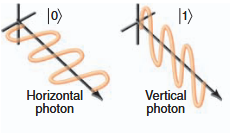
\includegraphics[width=0.5\linewidth]{images/physics/Photonen_Polarisierung.png}
    \caption{Enter Caption}
    \label{fig:enter-label}
\end{figure}
\cite{obrien_optical_2007}

2. Time-Bin-Encoding \\
Das Time-Bin-Encoding beschreibt die Kodierung der Quanteninformationen in verschiedenen Zeitfenstern, sogenannten "Time Bins". 
Ein Eintreffen des Photons in einem früheren Zeitfenster entspricht hierbei dem Zustand 0, ein späteres Eintreffen dem Zustand 1. Ein gleichzeitiges Eintreffen entspricht einer Superposition. \\ \cite{obrien_optical_2007}

3. Pfad-Kodierung (Dual Rail Encoding)\\
Bei der Pfad-Kodierung wird ein Qubit durch ein einzelnes Photon dargestellt, das sich in einem von zwei räumlich getrennten Pfaden befindet. Die Anwesenheit des Photons im ersten Pfad steht für den Zustand |0⟩, im zweiten Pfad für |1⟩. Befindet sich das Photon gleichzeitig in beiden Pfaden, entspricht das einer Superposition\\

Um logische Operationen auf solchen Qubits durchzuführen, nutzt man optische Elemente wie Strahlteiler (Beamsplitter), die das Photon auf beide Pfade verteilen können, sowie Phasenverschiebungselemente, die die relative Phase verändern. \\

Pfad- und Polarisationskodierung lassen sich außerdem mithilfe von Polarisations-Strahlteilern ineinander umwandeln, was eine flexible Nutzung beider Kodierungsarten erlaubt.  \cite{nielsen_michael_a_and_isaac_l_chuang_quantum_2010}\\\\
%Teil II, Kapitel 7.4

\subsubsection{Herausforderungen}
Die Herausforderung liegt bei der Realisierung effizienter Zwei-Qubit-Gatter, die für viele Quantenalgorithmen benötigt werden. Bei diesen Gattern hängt der Zustand eines Qubits von dem eines anderen ab, was eine starke Wechselwirkung zwischen den einzelnen Qubits erfordert. Wie zu Beginn dieses Abschnitts erwähnt, wechselwirken Photonen kaum - weder untereinander noch mit der Umwelt. \\
Ein gegenseitiger Wechselwirkungseffekt kann technisch zwar erreicht werden, jedoch ist dieser in allen bekannten Materialien extrem schwach, sodass für eine ausreichend hohe Wechselwirkung etwa 50 Photonen absorbiert werden würden. Da Quanteninformation bereits durch den Verlust einzelner Photonen zerstört wird, ist dieser Ansatz für Quantencomputer nicht geeignet. \\

Eine weitere Schwierigkeit bei der Umsetzung komplexer Quantenalgorithmen ist die Notwendigkeit einer großen Anzahl stabiler optischer Interferometer. Diese werden benötigt, um die Phasenzustände der Photonen und damit die gespeicherten Informationen gezielt zu verändern und auszulesen. Das Zusammenschalten von vielen Interferometern, sodass die Phasen stabil gehalten werden können, erfordert sehr viel Aufwand. \\


Abgesehen von den Herausforderungen der Realisierung von Zwei-Qubit-Gatter und der Skalierbarkeit des Zustandsraum erfüllen photonenbasierte Qubits die DiVincenzo-Kriterien sehr gut. Sie können zuverlässig in einen definierten Anfangszustand gebracht werden, sind nahezu ideal isoliert und können Ein-Qubit-Gatter einfach umsetzen. Mit geeigneten Strahlteilern und Polarisationsfiltern ist auch eine eindeutige Messung möglich. \\
Trotz der genannten Einschränkungen gelten photonische Systeme als vielversprechend. 
\cite{nielsen_michael_a_and_isaac_l_chuang_quantum_2010}
%Teil II, Kapitel 7.4




\subsection{Spin-Qubits}
\label{subsec: Spin-Qubits}
Spin-Qubits gehören zu den vielversprechendsten physikalischen Realisierungsformen von Qubits. Sie basieren auf dem quantenmechanischen Eigendrehimpuls, dem Spin, von Elektronen oder Atomkernen. Die beiden möglichen Orientierungen des Spins, üblicherweise als $\ket{\uparrow}$ (Spin-up) und $\ket{\downarrow}$ (Spin-down) bezeichnet, bilden die Basiszustände eines Qubits.

Die gezielte Kontrolle dieser Zustände erfolgt durch äußere Einflüsse, meist in Form elektromagnetischer Felder. Hierbei werden Mikrowellenimpulse oder lokal angelegte Magnetfelder genutzt, um mithilfe von Spinresonanz Zustandsänderungen zu induzieren.

In der Praxis kommen Spin-Qubits häufig in Halbleitern zum Einsatz. Quantendots dienen dabei als künstliche Atome, in denen einzelne Elektronen gefangen sind. Alternativ finden auch Defektzentren in Diamantstrukturen, etwa NV-Zentren, Anwendung. Diese Systeme bieten Potenzial für eine Integration in bestehende Halbleitertechnologien.

Ein bedeutender Vorteil von Spin-Qubits liegt in ihren vergleichsweise langen Kohärenzzeiten. Dadurch bleibt die Quanteninformation über relevante Zeitspannen hinweg erhalten, was sie für die praktische Nutzung besonders attraktiv macht.

Die Wechselwirkung zwischen mehreren Spin-Qubits wird typischerweise durch Austauschkopplung oder über gemeinsame Felder vermittelt. Diese Kopplung ist notwendig für die Umsetzung von Quantenlogikgattern, erfordert aber hochpräzise Steuerung und Isolation gegenüber Umwelteinflüssen.

Forschungsschwerpunkte liegen aktuell auf der Verbesserung von Kohärenzzeiten, der Entwicklung effizienter Fehlerkorrekturverfahren und der Skalierung zu größeren Systemen. Ziel ist es, auf dieser Grundlage robuste Quantenprozessoren zu realisieren \cite{nielsen_quantum_2010, Kapitel 7.7}.

\subsection{Neutralatom-Qubits}
\label{subsec: Neutralatom-Qubits}
Neutralatom-Qubits verwenden einzelne, elektrisch neutrale Atome als Träger von Quanteninformation. Diese Atome werden durch optische Fallen oder optische Gitter eingefangen und lassen sich auf engstem Raum präzise anordnen. Als Qubit-Zustände dienen dabei zwei ausgewählte hyperfeine Energieniveaus, die durch Kopplung zwischen Elektronen- und Kernspin entstehen.

Die Manipulation dieser Zustände erfolgt durch kohärente Laserpulse. Diese ermöglichen sowohl Zustandsübergänge als auch kontrollierte Wechselwirkungen zwischen benachbarten Atomen. Besonders relevant sind Rydberg-Zustände, bei denen sich ein Elektron in einem stark angeregten Zustand befindet.

Rydberg-Zustände zeichnen sich durch stark verstärkte Wechselwirkungen aus. Sie erlauben die Realisierung von Zwei-Qubit-Gattern über Mechanismen wie die Rydberg-Blockade, bei der bestimmte Übergänge durch das Vorhandensein eines benachbarten angeregten Atoms unterdrückt werden.

Ein großer Vorteil von Neutralatom-Qubits ist ihre hervorragende Skalierbarkeit. Optische Gitter ermöglichen die gleichzeitige Kontrolle von Tausenden Atomen mit hoher Reproduzierbarkeit und Homogenität. Auch die Kohärenzzeiten sind in vielen Szenarien konkurrenzfähig mit anderen Plattformen.

Gleichzeitig bestehen Herausforderungen bei der exakten Positionierung, der Einzeladressierung und der Minimierung störender Einflüsse wie Streulicht oder thermischen Fluktuationen. Hier konzentriert sich die aktuelle Forschung auf verbesserte Kontrollmechanismen und die Integration komplexerer Strukturen.

Neutralatom-Qubits ergänzen bestehende Plattformen sinnvoll. Ihre Kombination aus Skalierbarkeit, Präzision und Kohärenz macht sie zu einer zentralen Technologie für Quantencomputer und spezialisierte Quantensimulatoren.





\subsection{Diamantbasierte Qubits}
\label{subsec: Diamantbasierte Qubits}

Diamant bietet hervorragende physikalische Eigenschaften für Quantenanwendungen: das extrem steife Kristallgitter reduziert atomare Vibrationen, was das Material sehr robust macht. \\
Zusätzlich sorgt die große Bandlücke von 5,5 eV für das transparente Erscheinungsbild von Diamant, da fast das gesamte sichtbare Lichtspektrum nicht absorbiert wird. Das führt zu einer Reduktion von Störprozessen. \\
Darüber hinaus besteht natürlicher Kohlenstoff zu 98,9\% aus dem Isotop ${}^{12}C$, welches keinen Kernspin besitzt und damit zu das magnetische Rauschen besonders niedrig hält. Dadurch werden außergewöhnlich lange Spin-Kohärenzzeiten ermöglicht. \\

Diamantbasierte Qubits beruhen auf sogenannten Farbzentren, also winzigen Fehlstellen oder Verunreinigungen im Kristallgitter, die als stabile Elektronenspin-Systeme fungieren und sich dadurch gut als Qubits einsetzen lassen. Diese Farbzentren sind optisch aktive Defekte innerhalb der Bandlücke von Diamant und speichern Information typischerweise in der Spinprojektion entlang einer Kristallachse. \\

Bislang sind über 200 verschiedene Farbzentren bekannt, die alle durch unterschiedliche Kombinationen von Fremdatomen und Fehlstellen im Kohlenstoffgitter entstehen. Besonders bekannt ist dabei das Stickstoff-Fehlstellenzentrum (NV-Zentrum), welches aus einem Stickstoffatom und einer benachbarten Fehlstelle im Diamantgitter besteht. \\

Die Spin-Zustände des NV-Zentrums bilden ein Spin-Triplett mit drei Zuständen, die sich durch die Ausrichtung ihrer Spins unterscheiden: $ms = 0$ und $ms = \pm 1$
Für ein Qubit können beispielsweise die Niveaus $ms = 0$ und $ms = -1$ des Grundzustandes verwendet werden . \\
Die Elektronen im Grundzustand werden mit einem grünen Laser angeregt. Dabei zerfallen die Zustände $ms = \pm 1$ schneller in den Grundzustand $ms=0$ zurück, sodass nach mehreren Zyklen die gesamte Besetzung sich im Zustand $ms=0$ befindet. Dies entspricht dem definierten Startzustand. \\

Durch die Manipulation des Zustands mit einem magnetischen Feld mit der Mikrowellenfrequenz von 2.88GHz kann kontrolliert zwischen den Zuständen gewechselt werden und so Quantenoperationen ausgeführt werden. \\

Herausforderungen  bei diamantbasierten Qubits sind die zuverlässige Herstellung hochkohärenter Qubits sowie die Skalierbarkeit der benötigten photonischen Strukturen. Zusätzlich begrenzt der hohe Brechungsindex von Diamant die Photoneneinfangrate außerhalb des Kristalls, was die Verbindung der Qubits mit optischen Netzwerken erschwert. Auch der Mangel an ultra-hochwertigen Diamant-Dünnschichten erschwert die Fertigung. \\

Diamantbasierte Qubits, insbesondere auf Basis von NV-Zentren, erfüllen die DiVincenzo-Kriterien in weiten Teilen sehr gut. Sie bieten einen klar definierbaren und optisch adressierbaren Zustandsraum, ermöglichen durch optisches Pumpen einen reproduzierbaren Startzustand und zeichnen sich durch außergewöhnlich lange Kohärenzzeiten aus, was einen entscheidender Vorteil gegenüber vielen anderen Qubit-Plattformen darstellt. Ein-Qubit-Operationen lassen sich präzise über Mikrowellensteuerung realisieren, und auch die Messung einzelner Qubits ist über Fluoreszenzkontraste zuverlässig möglich.  \\
Trotz der Herausforderungen der Skalierbarkeit und Herstellung identischer NV-Zentren sowie der Implementierung effizienter Zwei-Qubit-Gatter gilt Diamant als vielversprechende Plattform für Quanteninformationsverarbeitung, vor allem in Bereichen mit Fokus auf Langzeitstabilität und Kohärenz. 


\cite{ulanov_diamantbasierte_2025}


\printbibliography
